\documentclass[11pt]{article}
\usepackage[utf8]{inputenc}
\usepackage{amssymb, amsmath, amsthm, changepage, graphicx, caption, subcaption}

\graphicspath{{./images/}}

\title{PUMP II Problem Set 2}
\author{Nick Coballe, Krishna Cheemalapati, Daniel Xu}

\newcommand{\bproof}{\begin{proof}
$ $ \\
\begin{adjustwidth}{3em}{0pt}
}

\newcommand{\eproof}{\end{adjustwidth}
\end{proof}}

\begin{document}
\maketitle

\begin{flushleft}

1. a) \bigskip

\bproof
	Let $q(x) := 0$ and $r(x) := P_1(x)$ \\
	Thus $P_1 = 0(P_2) + P_1$ \\
	And by assumption $deg(r) = deg(P_1) < deg(P_2)$
\eproof

b) \bigskip

\bproof
	Let $P_1(x) = a_0 + a_1x + \ldots + a_nx^n$ and $P_2(x) = b_0 + b_1x + \ldots + b_mx^m$ \\ \bigskip
	
	Case 1: $n = m$ \\
	$P_1(x) = \frac{a_n}{b_m}P_2(x)+(a_0- \frac{a_n}{b_m} b_0) + (a_1- \frac{a_n}{b_m} b_1)x + \ldots + (a_{m-1}- \frac{a_n}{b_m} b_{m-1})x^{m-1}$ \\
	Thus $q(x) := \frac{a_n}{b_m}$ and $r(x) := (a_0- \frac{a_n}{b_m} b_0) + (a_1- \frac{a_n}{b_m} b_1)x + \ldots + (a_{m-1}- \frac{a_n}{b_m} b_{m-1})x^{m-1}$ \
	and $deg(r) = deg(m) - 1 < deg(m)$ as desired. \\ \bigskip
	
	Case 2: $n > m$ \\
	We will induct on $n$ \\
	Base Case: $n = 1$ and $m = 0$ \\
	\begin{center}
	$P_1(x) = \frac{1}{b_0} P_1(x)P_2(x)$ \\
	$q(x) := \frac{1}{b_0} P_1(x)$ and $r(x) := 0$ \\
	\end{center}
	Thus the base case is true. \\
	Inductive Step: $k = n+1$ \\
	Let $q(x) = \frac{a_{n+1}}{b_m} x^{n+1-m} + q'(x)$ where $q'(x)$ is some polynomial.
	\begin{align*}
	P_1(x) &= (\frac{a_{n+1}}{b_m} x^{n+1-m} + q'(x))P_2(x) + r(x) \\
	P_1(x) - (\frac{a_{n+1}}{b_m} x^{n+1-m})P_2(x) &= q'(x)P_2(x) + r(x)
	\end{align*}
	Because $P_1(x)$ and $(\frac{a_{n+1}}{b_m} x^{n+1-m})P_2(x)$ have the same degree and leading coefficient, their difference, at most, is of degree n. \\
	Thus we can set some polynomial \\ 
	\begin{center}
	$P_1'(x) := P_1(x) - (\frac{a_{n+1}}{b_m} x^{n+1-m})P_2(x)$\\
	$P_1'(x) = q'(x)P_2(x) + r(x)$ \\
	\end{center}
	But because $deg(P_1') \leq n$ by the induction hypothesis, $q'(x)$ and $r(x)$ exists.
\eproof

c) \bigskip

\bproof
	\begin{align*}
	P_1 &= qP_2 + r \\
	P_1 &= \tilde{q}P_2 + \tilde{r}
	\end{align*}
	Taking the difference of these equations leaves us with
	\begin{align*}
	0 = (q - \tilde{q})P_2 +r - \tilde{r}
	\end{align*}
	Because $deg((q - \tilde{q})P_2) > deg(r)$ and $deg((q - \tilde{q})P_2) > deg( \tilde{r})$ then $(q - \tilde{q})P_2 \notin span(r, \tilde{r})$ \\
	Thus to equal the zero polynomial, $(q - \tilde{q})P_2 = 0$ and since $P_2 \neq 0$ then $q - \tilde{q} = 0$, leaving us with $q = \tilde{q}$ \\
	Because $(q - \tilde{q})P_2 = 0$, then $r - \tilde{r} = 0$ and thus $r = \tilde{r}$ as desired.
\eproof

\newpage

d) \bigskip

\bproof
	$\Rightarrow$ \\
	Using Theorem 1, we can set $P_2(x) = x - \alpha$ and thus any polynomial of positive degree, $P_1$ can be written
	\begin{align*}
	P_1(x) &= q(x)(x - \alpha) + r(x) \\
	P_1(\alpha) &= q(\alpha)(\alpha - \alpha) + r(\alpha) \\
	0 &= r(\alpha)
	\end{align*}
	Because $deg(r) < deg(x- \alpha) = 1$, $r$ must be a constant, and since it maps $\alpha$ to zero, it must be the zero function. Then $P_1(x) = q(x)(x - \alpha)$ and thus $(x - \alpha)$ is a factor of $P_1$. \\ \bigskip
	$\Leftarrow$ \\
	By assumption $P(x) = q(x)(x - \alpha)$
	\begin{align*}
	P(\alpha) &= q(\alpha)(\alpha - \alpha) \\
	&= q(\alpha)(0) \\
	&= 0 
	\end{align*}
	And thus, $\alpha$ is a root of $P$.
	
\eproof

\newpage

2. a) \bigskip \\
\begin{figure}[h]
\centering

	\begin{subfigure}[b]{0.3\textwidth}
	\centering
	
	\label{fig:i}
	\caption{$r=1$}
	\end{subfigure}
	\hfill
	\begin{subfigure}[b]{0.3\textwidth}
	\centering
	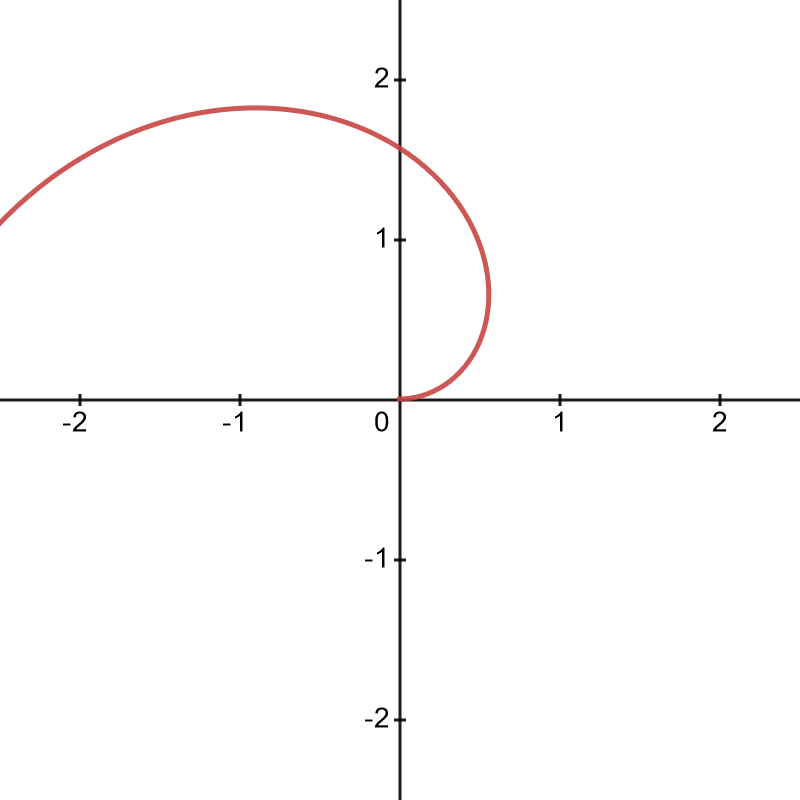
\includegraphics[width=\textwidth]{requalstheta.png}
	\label{fig:ii}
	\caption{$r=\theta$}
	\end{subfigure}
	\hfill
	\begin{subfigure}[b]{0.3\textwidth}
	\centering
	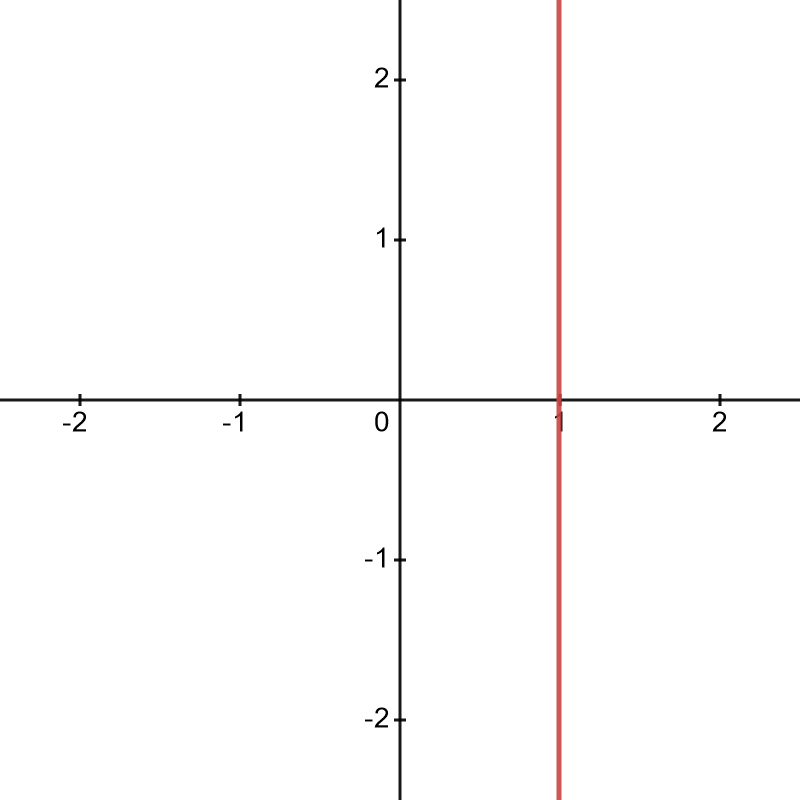
\includegraphics[width=\textwidth]{requalssecanttheta.png}
	\label{fig:iii}
	\caption{$r=sec(\theta)$}
	\end{subfigure}
	
\end{figure}

b) \bigskip

\bproof
	\begin{align*}
	d^2 &= (x_1-x_2)^2 + (y_1-y_2)^2 \\
	&= x_1^2 -2x_1x_2 + x_2^2 + y_1^2 -2y_1y_2 + y_2^2 \\	
	\begin{split}
	&= r_1^2cos^2(\theta_1) -2r_1cos(\theta_1)r_2cos(\theta_2) + r_2^2cos^2(\theta_2) + r_1^2sin^2(\theta_1) \\
	& \quad -2r_1sin(\theta_1)r_2sin(\theta_2) + r_2^2sin^2(\theta_2) \\
	\end{split} \\
	\begin{split}
	&= r_1^2(cos^2(\theta_1) + sin^2(\theta_1)) + r_2^2(cos^2(\theta_2) + sin^2(\theta_2)) \\
& \quad -2r_1r_2(cos(\theta_1)cos(\theta_2) + sin(\theta_1)sin(\theta_2))
	\end{split} \\
	&= r_1^2 + r_2^2 -2r_1r_2cos(\theta_1 - \theta_2)
	\end{align*}
\eproof

\newpage

c) \bigskip

\bproof
	\begin{align*}
	1 &= d_1d_2 \\
	1 &= d_1^2d_2^2 \\
	1 &= (r^2 + 1^2 -2rcos(\theta))(r^2 + (-1)^2 -2rcos(\theta - \pi)) \\
	1 &= (r^2 + 1 -2rcos(\theta))(r^2 + 1 +2rcos(\theta)) \\
	\begin{split} 0 &=
	r^4 + r^2 + 2r^3cos(\theta) + r^2 + 2rcos(\theta) - 2r^3cos(\theta)\\ & - 2rcos(\theta) - 4r^2cos^2(\theta) \end{split} \\
	0 &= r^4 + 2r^2 - 4r^2cos^2(\theta) \\
	0 &= r^2 + 2 - 4cos^2 \\
	2(2cos(\theta) -1) &= r^2 \\
	2cos(2\theta) &= r^2
	\end{align*}			
\eproof

d) \bigskip
\begin{figure}[h]
\centering
	\begin{subfigure}[b]{0.3\textwidth}
	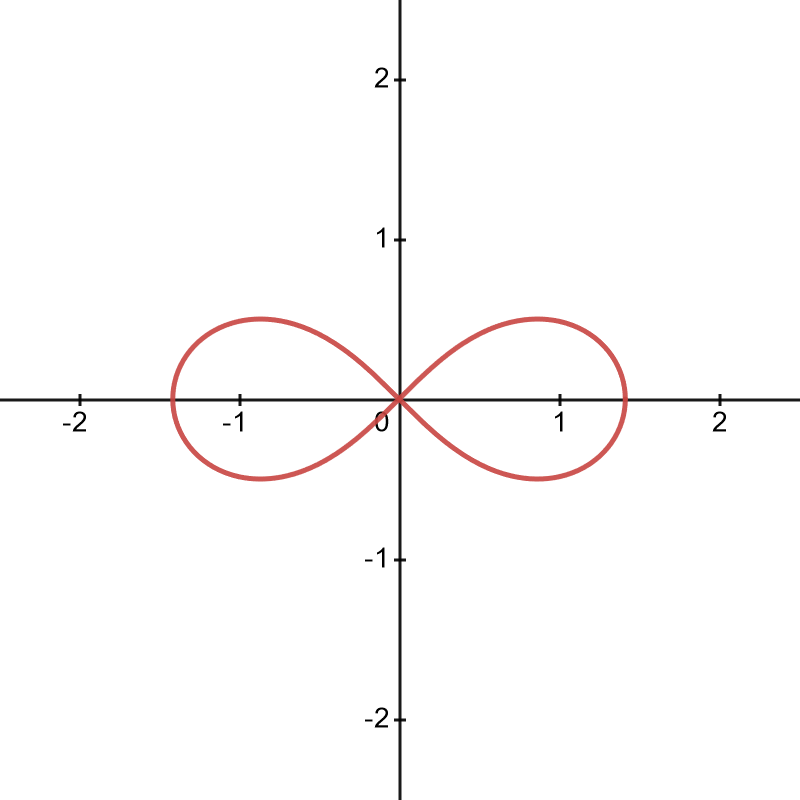
\includegraphics[width=\textwidth]{r=sqrt2cos2theta.png}
	\caption{$r^2=2cos(2\theta)$}
	\end{subfigure}
\end{figure}

\newpage

e) \bigskip

\begin{align*}
	r^2 &= 2cos(2\theta) \\
	r^2 &= 2cos^2(arccos(\frac{x}{r})) -2sin^2(arcsin(\frac{y}{r}))\\
	r^2 &= 2\frac{x^2}{r^2} -2\frac{y^2}{r^2}	 \\
	r^4 &= 2x^2 -2y^2 \\
	(x^2+y^2)^2 &= 2x^2 -2y^2
\end{align*}

\newpage

3. a) \bigskip

\bproof
	\begin{align*}
	f_{\vec{u}}(\vec{v} + \vec{w}) &= \begin{pmatrix}
	u_2(v_3 + w_3) - u_3(v_2 + w_2) \\
	u_3(v_1 + w_1) - u_1(v_3 + w_3) \\
	u_1(v_2 + w_2) - u_2(v_1 + w_1)
	\end{pmatrix} \\
	&= \begin{pmatrix}
	u_2v_3 + u_2w_3 -u_3v_2 -u_3w_2 \\
	u_3v_1 + u_3w_1 -u_1v_3 -u_1w_3 \\
	u_1v_2 + u_1w_2 -u_2v_1 -u_2w_1 \\
	\end{pmatrix} \\
	&= \begin{pmatrix}
	u_2v_3 -u_3v_2 \\
	u_3v_1 -u_1v_3 \\
	u_1v_2 -u_2v_1 \\
	\end{pmatrix}
	+ \begin{pmatrix}
	u_2w_3 -u_3w_2 \\
	u_3w_1 -u_1w_3 \\
	u_1w_2 -u_2w_1 \\
	\end{pmatrix} \\
	&= f_{\vec{u}}(\vec{v}) + f_{\vec{u}}(\vec{w})
	\end{align*}
	\begin{align*}
	f_{\vec{u}}(\lambda \vec{v}) &= \begin{pmatrix}
	u_2(\lambda v_3) - u_3(\lambda v_2) \\
	u_3(\lambda v_1) - u_1(\lambda v_3) \\
	u_1(\lambda v_2) - u_2(\lambda v_1) \\
	\end{pmatrix} \\
	&= \begin{pmatrix}
	\lambda (u_2v_3-u_3v_2) \\
	\lambda (u_3v_1-u_1v_3) \\
	\lambda (u_1v_2-u_2v_1) \\
	\end{pmatrix} \\
	&= \lambda \begin{pmatrix}
	u_2v_3-u_3v_2 \\
	u_3v_1-u_1v_3 \\
	u_1v_2-u_2v_1 \\
	\end{pmatrix} \\
	&= \lambda f_{\vec{u}}(\vec{v})
	\end{align*}

\eproof

\newpage

b)  \bigskip

\bproof
	\begin{align*}
	f_{\vec{u} + \vec{v}}(\vec{w}) &= \begin{pmatrix}
	(u_2 + v_2)w_3 -(u_3 + v_3)w_2 \\
	(u_3 + v_3)w_1 -(u_1 + v_1)w_3 \\
	(u_1 + v_1)w_2 -(u_2 + v_2)w_1 \\
	\end{pmatrix} \\
	&= \begin{pmatrix}
	u_2w_3 + v_2w_3 -u_3w_2 -v_3w_2 \\
	u_3w_1 + v_3w_1 -u_1w_3 -v_1w_3 \\
	u_1w_2 + v_1w_2 -u_2w_1 -v_2w_1 \\
	\end{pmatrix} \\
	&= \begin{pmatrix}
	u_2w_3 -u_3w_2 \\
	u_3w_1 -u_1w_3 \\
	u_1w_2 -u_2w_1 \\
	\end{pmatrix}
	+ \begin{pmatrix}
	v_2w_3 -v_3w_2 \\
	v_3w_1 -v_1w_3 \\
	v_1w_2 -v_2w_1
	\end{pmatrix} \\
	&= f_{\vec{u}}(\vec{w}) + f_{\vec{v}}(\vec{w})
	\end{align*}			
	
	\begin{align*}
	f_{\lambda \vec{u}}(\vec{v}) &= \begin{pmatrix}
	(\lambda u_2)v_3 -(\lambda u_3)v_2 \\
	(\lambda u_3)v_1 -(\lambda u_1)v_3 \\
	(\lambda u_1)v_2 -(\lambda u_2)v_1 \\
	\end{pmatrix} \\
	&= \begin{pmatrix}
	\lambda (u_2v_3 - u_3v_2) \\
	\lambda (u_3v_1 - u_1v_3) \\
	\lambda (u_1v_2 - u_2v_1) \\
	\end{pmatrix} \\
	&= \lambda \begin{pmatrix}
	(u_2v_3 - u_3v_2) \\
	(u_3v_1 - u_1v_3) \\
	(u_1v_2 - u_2v_1) \\
	\end{pmatrix} \\
	&= \lambda f_{\vec{u}}(\vec{v})
	\end{align*}
\eproof

\newpage

c) \bigskip

\bproof
	\begin{align*}
	(f_{\vec{u}} \circ  f_{\vec{v}})(\vec{w}) - (f_{\vec{v}} \circ  f_{\vec{u}})(\vec{w}) &= f_{\vec{u}}(f_{\vec{v}}(\vec{w})) - f_{\vec{v}}(f_{\vec{u}}(\vec{w})) \\
	\begin{split}
	&= \begin{pmatrix}
	u_2v_1w_3 - u_2v_2w_1 - u_3v_3w_1 + u_3w_1w_3 \\
	u_3v_2w_3 - u_3v_3w_2 - u_1w_1w_1 + u_1v_2w_1 \\
	u_1v_3w_1 - u_1v_1w_3 - u_2v_2w_3 + u_2v_3w_2
	\end{pmatrix} \\
	& \quad - \begin{pmatrix}
	u_1v_2w_2 - u_2v_2w_1 - u_3v_3w_1 + u_1v_3w_3 \\
	u_2v_3w_3 - u_3v_3w_2 - u_1v_1w_2 + u_2v_1w_1 \\
	u_3v_1w_1 - u_1v_1w_3 - u_2v_2w_3 + u_3v_2w_2 \\
	\end{pmatrix} 
	\end{split} \\
	&= \begin{pmatrix}
	u_2v_1w_3 + u_2v_1w_3 - u_1v_2w_2 - u_1v_3w_3 \\
	u_3v_2w_3 + u_1v_2w_1 - u_2v_3w_3 - u_2v_1w_1 \\
	u_1v_3w_1 + u_2v_3w_2 - u_3v_1w_1 - u_3v_2w_2 \\
	\end{pmatrix}\\
	&= (f_{\vec{u}\times \vec{v}}(\vec{w})
	\end{align*}


\eproof

d) \bigskip

\bproof
	$\Rightarrow$ \\
	If \\
	\begin{align*}
	f_{\vec{u}} \begin{pmatrix}
	1 \\
	0 \\
	0 \\
	\end{pmatrix} &= \vec{0} \\
	\begin{pmatrix}
	u_2(0) - u_3(0) \\
	u_3(1) - u_1(0) \\
	u_1(0) - u_2(1) \\
	\end{pmatrix} &= \begin{pmatrix}
	0 \\
	0 \\
	0 \\
	\end{pmatrix}
	\end{align*}
	Then $u_3 = 0$ and $u_2 = 0$ and \\
	\begin{align*}
	f_{\vec{u}} \begin{pmatrix}
	0 \\
	1 \\
	0 \\
	\end{pmatrix} &= \vec{0} \\
	\begin{pmatrix}
	u_2(0) - u_3(1) \\
	u_3(0) - u_1(0) \\
	u_1(1) - u_2(0) \\
	\end{pmatrix} &= \begin{pmatrix}
	0 \\
	0 \\
	0 \\
	\end{pmatrix}
	\end{align*}
	then $u_1 = 0$ and thus $\vec{u} = \vec{0}$ \\ \bigskip
	$\Leftarrow$ \\
	\begin{align*}
	f_{\vec{u}}(\vec{v}) &= \begin{pmatrix}
	0w_3 - 0w_2 \\
	0w_1 - 0w_3 \\
	0w_2 - 0w_1 \\
	\end{pmatrix} \\
	&= \begin{pmatrix}
	0 \\
	0 \\
	0 \\
	\end{pmatrix}
	\end{align*}
	Thus $f_{\vec{u}}(\vec{v}) = 0$

\eproof

\end{flushleft}
\end{document}